\chapter{}

\section*{Из воспоминаний М.В. Миникса}

\textbf{О хозяйстве и работниках Дома у Красных ворот\protect\footnote{Пишу все, что вспомнил и как помню. Другие могут рассказать о том же, но по-своему. Мне кажется, это (такие повторы)~-- не страшно.} (<<дома образцового содержания>>).} Нашим замечательным Управдомом долгие годы был Иван Максимович Калиш. Сохранилась фотография, на которой изображена скамейка в садике нашего Дома, а на ней мы с папой, Иван Максимович и А.И. Кузнецов. Подобные фотографии есть и в других семьях, поскольку И.М. Калиш со многими жильцами дома был в приятельских и даже дружеских отношениях. Потом его место заняла Александра Никитична Давыдова, которая уже в 50-е годы поселилась в 6-ом подъезде нашего Дома.

Все аварийные ситуации в Доме успешно побеждали свой мастер на все руки (слесарь-сантехник, электрик и проч.) N.N. Барский и его помощница Наташа. Если не ошибаюсь, в конце сороковых годов дочь Барского вышла замуж за старшего сына полковника Иванцова из 5-го подъезда. Был и свой столяр, который с семьей жил в подвале 5-го подъезда (за Красным уголком).

Весьма авторитетной фигурой для нас, мальчишек Дома, был Главный дворник Дядя Павел. А был еще второй дворник N. Шапиро.

В Доме была оборудована собственная котельная для обогрева квартир зимой, а в ванных вода нагревалась с помощью газовой горелки фирмы <<Юнкерс>>, что казалось забавным для детей войны. Некоторые жильцы у себя в квартирах сделали отвод горячей воды из ванной на кухню (по тем временам~-- чудеса да и только!). Кто был Главным истопником~-- не помню, но у него было два сына: Ислам и  Мареф. Вход в котельную был с заднего двора, а окна из нее выходили в подвал под вторым подъездом. Как-то летом, уже в конце 50-х или в начале 60-х, из этого подвала появилась перепачканная мордашка очаровательной девицы лет трех, которая доверительно обратилась ко мне с жалобой на жизнь: <<Я один, совсем один... мне так грустно...>> (детей во дворе~-- никого; это была дочка одной из сестер Гущиных, которая вышла замуж в Румынии и гостила у родных).

В Доме работали лифты (в 30-х годах это было событием). Вначале лифтеры круглосуточно дежурили в каждом подъезде. Затем, по два лифтера обслуживали все лифты. Их штаб-квартира располагалась в сторожке, а она~-- в подворотне.

Внутридомный Детсад (подробнее см. выше~-- воспоминания О.А. Гриневского) вначале размещался во 2-м подъезде, а затем  расширился за счет места для квартир первого этажа 3-го (окна на улицу) и 4-го (окна во двор) подъездов. Для ребят всех возрастов организовывались экскурсии по Москве.

В Доме еще до войны работал стол продовольственных заказов. Для постоянных клиентов в стену подворотни был встроен блок из двадцати с лишним сейфов-ячеек, в которые загружали готовые заказы, а каждый из клиентов имел ключ от своей ячейки. Привозили заказы на открытом пикапе. Мы помогали его разгружать; за это нас катали по двору (по улице нельзя!).

Пункт приема в стирку и выдачи чистого белья был организован в подвале 1-го подъезда, а затем перекочевал в подвал под 7-ым подъездом. В этом подвале в разные времена работала столовая (был и буфет).

Собственная снеготаялка располагалась около ворот заднего двора, недалеко от котельной. Мусоросборник и мусоросжигалка также была на заднем дворе (около окон 3-го подъезда).

Особое место занимал и особую роль в жизни Дома играл Красный уголок, расположенный в подвале 5-го подъезда. В нем занимались самыми разнообразными делами и развлекались:

\begin{itemize}
\item проводились собрания жильцов, занятия Ликбеза, выступали агитаторы в период проведения первых послевоенных выборов, готовились стенгазеты;
\item работали различные кружки: радиолюбителей, хоровой, драматический, моего сына учили даже играть на фортепиано, правда, не очень успешно;
\item иногда <<крутили>> кино, проходили концерты художественной самодеятельности;
\item работала библиотека;
\item можно было поиграть в бильярд, в настольные игры;
\item и многое-многое другое.
\end{itemize}

Это все были замечательные особенности Дома у Красных ворот.

Были и свои казусы:
\begin{itemize}
\item маленькие, в некоторых квартирах~-- крохотные уборные;
\item кухни трех размеров: крохотные, небольшие и побольше (до 8-9 метров);
\item во многих квартирах были предусмотрены шкафы-холодильники (с окошком на улицу), во многих~-- нет;
\item в одних квартирах были балконы, в других~-- нет, например на 3-м этаже 3-го подъезда: в кв. 35 был огромный балкон, а в кв. 34 и 36 балконов не было;
\item в <<левых>> (при подъеме по лестнице~-- налево) квартирах 3-го подъезда были затемненные комнаты и кухни (виноват странный выступ~-- квартиры 2-го подъезда). 
\end{itemize}

Я уже не говорю о том, как Дом образцового содержания пострадал за свои привилегии, сколько людей~-- не только Наркоминдельцев~-- погибло в сталинских застенках.

\newline

\textbf{Хорошие люди (из книжки <<О людях дома у Красных ворот>>).} Хороших людей в нашем доме было, конечно, больше, чем упомянуто в этих воспоминаниях. Запомнилось то, что забыть нельзя, да и не хочется.

\newline

Нашими ближайшими соседями были Кузнецовы: Алексей Ильич, Варвара Николаевна, ее дочь от первого брака Александра Гавриловна и внучка Ия Бабенко, одноклассница моего брата Абы (1924 г.р.). Самой близкой была баба Варя, добрейший человек, истинная христианка. На Пасху она угощала нас куличом, а во время войны~-- блинчиками из картофельных очисток. Она почему-то любила сажать меня на стол, лет до пяти. До сих пор чувствую ее теплоту.

\newline
Рядом с ними жили Е. В. Голубева~-- мудрая, очень выдержанная, интеллигентная женщина, и ее сыновья: Юра (погиб на войне) и Сережа (см. раздел VIP) Дивильковские. Как дорогую реликвию храню книгу «Славные большевички», которую с теплой надписью подарила моей маме Елена Васильевна. В этой книге она написала о своей маме, Марии Петровне Голубевой (Ясневой), члене партии с 1901 года, которая всю жизнь была честным и бескорыстным работником. Ее хорошо знал и ценил В. И. Ленин, тепло принимали члены его большой и дружной семьи (в начале века).

\newline

На шестом этаже, над нами, жили Дмитрий Афанасьевич Кузнецов~-- профессор, доктор, проректор Менделеевки, его жена Мария Леоновна~-- доцент того же института, их дети Галя (Ая) и Леончик.



В тяжелые послевоенные годы, когда мы с мамой жили впроголодь, и о покупке чего-либо из вещей не могло быть  и  речи,  Мария Леоновна или Леончик периодически приносили мне то рубашку, то костюм, то свитер. Все вычищенное, выглаженное и аккуратно сложенное. Однажды кто-то из них принес толщенное, тяжеленное пальто.

Через несколько дней к нам спустился Дмитрий Афанасьевич. В руках у него было шикарное, на мой взгляд, зимнее пальто с каракулевым воротником. И вот этот большой ученый и большой человек со смущенным видом стал объяснять мне, паршивому мальчишке (а был я, действительно, 

\newgeometry{left=0mm, right=0mm, top=0mm, bottom=0mm}

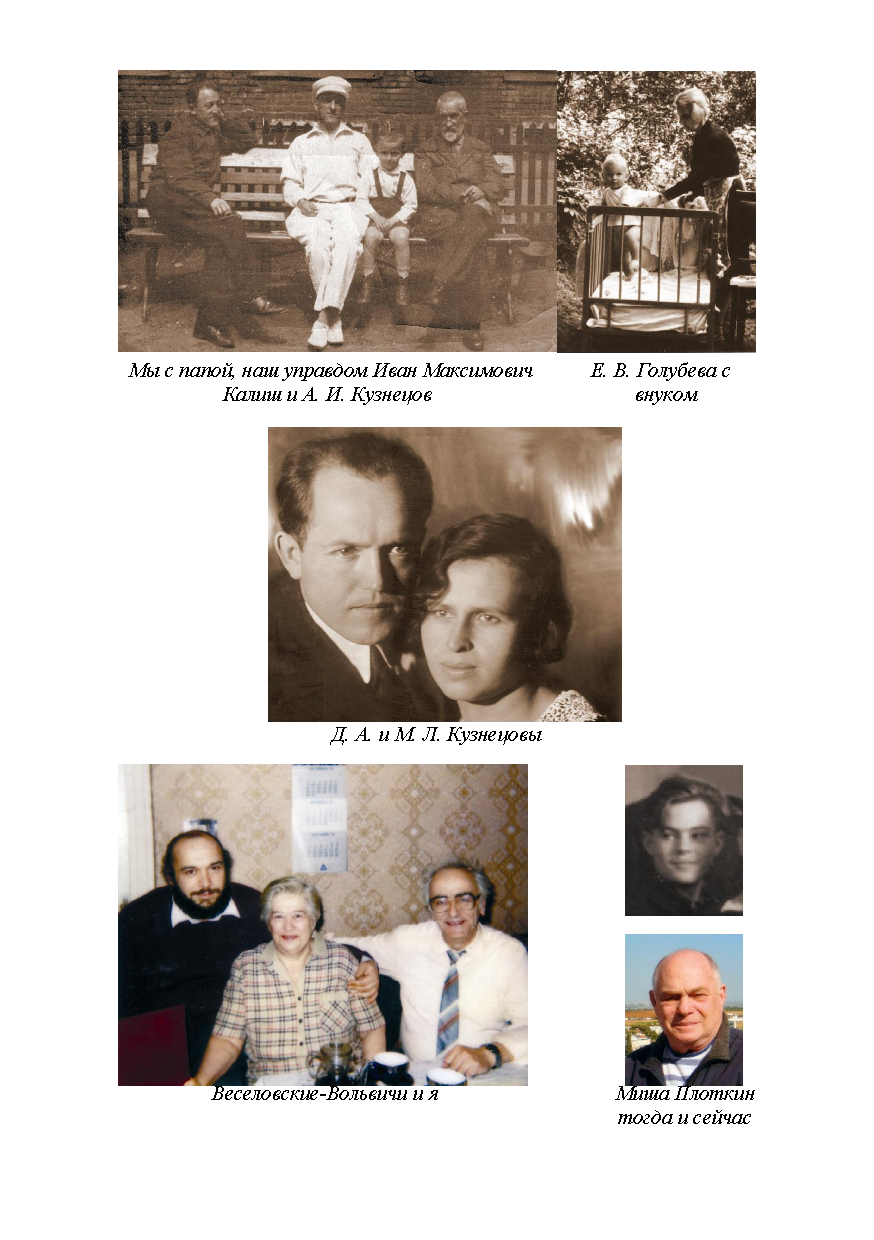
\includepdf[pages=-]{inc/fragment.pdf}

\restoregeometry

\noindentне сахар), что домочадцы случайно отдали важную для охоты (или рыбалки?) одежку и что он извиняется передо мной (!), что просит меня (!) принять, вместо того~-- это, правда~-- хорошее, пальто.



Такое невообразимое поведение на всю жизнь осталось для меня уроком такта и благородства.

\newline

В нашем же подъезде, на пятом этаже, жили Александровские: Андрей Сергеевич, Мария Осиповна и Лёлька~-- моя сверстница (о ней~-- отдельно). Родители Лёльки были высокообразованными людьми с широким кругом интересов. В доме у них была какая-то особая атмосфера. Там никому не пришло бы в голову громко разговаривать или ругаться. В этом доме я впервые услышал качественные записи музыкальной классики в превосходном, по тем временам, воспроизведении, увидел хорошие репродукции великих картин. Видимо, есть доля вины этих людей в том, что через несколько лет я стал «гурманом» в соответствующих областях культуры.

\newlin

Ирина Сергеевна Веселовская из второго подъезда относилась к промежуточному поколению (1926 или 1927 г. р.): между «старшими ребятами» и сверстниками моего брата. Наши дети были одногодками, но Лехи, увы, уже нет. Сразу после окончания института она попала в хозяйство Д. Ф. Устинова, который ее знал и ценил; многие годы руководила самым «хлебным» отделом – комплектации. Беда в том, что она была чрезвычайно честным человеком\protect\footnote{Она никогда не принимала никаких проявлений благодарности, даже искренних, даже совсем недорогих, не пользовалась обширными деловыми связями, даже в очень важных для себя случаях.} , поэтому на пенсии ей было очень трудно. Запасов (не только денег, но и вещей) не было, у Лехи не ладилось, но она всегда оставалась гордым, приветливым, очень надежным человеком; конечно же, никому никогда и не на что не жаловалась, даже перед смертью. 

\newline

Александр Абрамович Листенгордт (пятый подъезд), полковник госбезопасности, был добрейшим, наипорядочнейшим человеком, поэтому, видимо, его из центрального аппарата  сослали начальником лагеря  в Сибирь, где он жутко маялся с пузом (язва?). Знаменит он был тем, что, единственный из всего начальства, мог безбоязненно (без охраны!) ходить по зоне в любое время суток.


Старший его сын Володя~-- наш сверстник~-- был тоже добрым, но не очень счастливым человеком. Рано ушел из жизни. Младший сын, Фелюша~--  красивый, талантливый мальчик, хорошо учился, выступал по Всесоюзному радио. Стал крупным инженером, работал в оборонке.

\newline

Два года я учился в одном классе с Мишей Плоткиным (второй подъезд), который накануне Войны был знаменит на весь двор, поскольку владел единственным в мире (мы были в этом уверены) низким красным двухколесным велосипедом на широченных шинах (почти мотоцикл). В школе его не только любили, но и уважали: он был старостой класса, а его хотели выбрать еще и комсоргом. Позже он не раз прославлялся в науке, преподавании и в общественно-полезной деятельности, но, может быть, самой замечательной педагогической победой его было занятие с ребятами хоккеем на льду уже в ранге директора школы!

В конце 2009 года произошла знаменательная встреча (через 50 лет после предыдущей): Плоткина и Миникса с супругами и Светлану Сергеевну Моргунову пригласила к себе Элла Исааковна Певзнер (уроженка нашего дома, четвертый подъезд) – уникальный человек, известный в Европе энтузиаст и пропагандист Советской культуры и быта (ее фотографии см. на стр. 33 и 144).


\noindent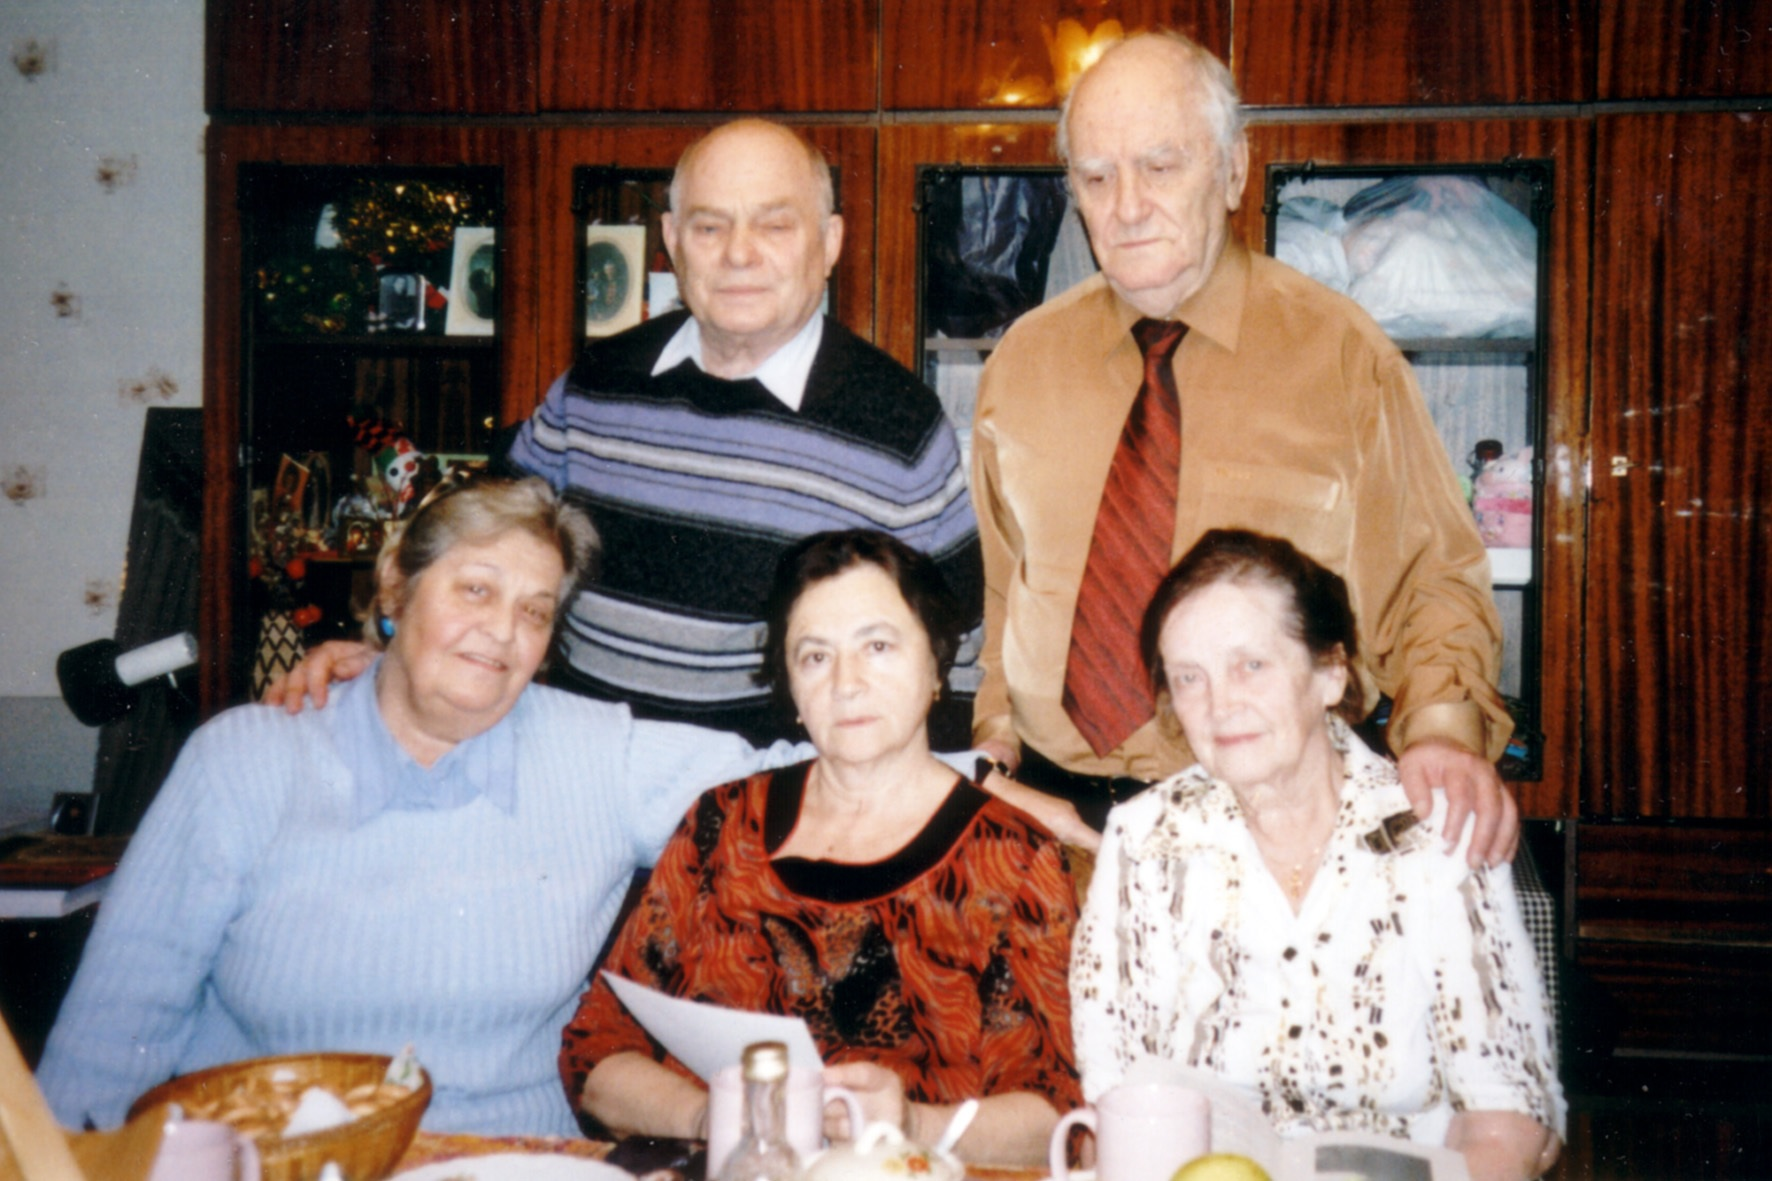
\includegraphics[width=\textwidth]{inc/toAppMinix.jpg}

Только что из книги З. Шейниса узнал о жуткой судьбе отца Миши~-- Марка Абрамовича Плоткина, заместителя заведующего правовым отделом Наркоминдела, члена партии с 1917 г. Один «хороший человек», друг Берии, зам. наркома НКИД Деканозов, пригласил его вечером на беседу, с которой он не вернулся, другой~-- Молотов~-- следующим утром вызывал его из дома для доклада: «Где он?». Вот в такие иезуитские игры играли сатрапы Сталина. М. А. Плоткин в 1939 году был расстрелян как враг народа. В 1956 г. полностью реабилитирован «за отсутствием состава преступления».  

\newline

Во втором подъезде жила удивительная женщина и великолепный врач Эсфирь Яковлевна Бару. Она в прямом смысле слова~-- спасла нашего сына. У жены была послеродовая грудница; в роддоме болезнь запустили настолько, что жену с сыном пришлось переводить в другую больницу на операцию. В этой больнице грубо нарушили режим кормления новорожденного ребенка, в результате у него развилась гипотрофия в очень тяжелой форме. Это обнаружила Эсфирь Яковлевна, которая проявила чудеса профессионализма и человеческого участия, чтобы спасти ребенка. Низкий ей поклон.

\newline

Марию Михайловну Гюнтер из нашего подъезда я в течение десятилетий периодически встречал на территории Донского крематория, где похоронены ее муж и старший сын, ушедшие из жизни один за другим. Теперь на памятнике и её фотография. Всегда подхожу к ним.

Помню, как Мария Михайловна получала уроки финансового мастерства от моего отца. Даже в очень преклонном возрасте она оставалась красивой женщиной. Я рад, что успел сказать ей об этом.
    
Очень симпатичным мне человеком был Ю. Д. Райский (седьмой, затем четвертый подъезд), но после детства мы встречались, в  основном, случайно. Вот почему. Более поздним моим друзьям\protect\footnote{Б. И. Моргунов, наоборот, относится к ранним друзьям (года с 48-го~-- 49-го), но это совсем другой случай~-- наши семьи, с пафосом говоря, проросли друг в друга, начиная с отцов и кончая детьми. На внуков, правда, это уже не распространяется.}  мне уже было, что предъявить, а в «Юрин период» я еще не созрел, не сформировался, поэтому был ему не интересен… и наши пути разошлись, хотя он был на нашей свадьбе, наши жены вместе гуляли с детьми, он тепло поддержал меня при неприятностях в институте, где он работал. То же относится и к некоторым другим друзьям той поры, вернее~-- приятелям.


Отдельно хочу сказать о человеке, которого мои родители знали с середины 20-х годов по первому дому НКИД\protect\footnote{Она знала многих наркоминдельцев в нашем доме, была частым гостем у нас и у них.}, а я с послевоенного времени – о Марии Михайловне Олькеницкой. Она была красивой, энергичной женщиной, незаурядным, сложным человеком, порой нетерпимым, противоречивым, всегда интересующимся всем, почти без исключения.
 
Выпускник экономического факультета МГУ, она с восхищением слушала лекции Н. И. Бухарина, видела и слышала Маяковского, Есенина, Северянина, Сашу Черного, великих актеров и писателей того и более позднего времени, знала многих художников, даже, кажется, Коровина. Очень интересно рассказывала о событиях и о людях. У меня хранятся подаренные ею альбомы И. Левитана, М. Врубеля, В. Серова  1957- 1959 годов выпуска\protect\footnote{Два последних с хорошими наклейными цветными иллюстрациями (как встарь в «Академии») – не хуже, чем в Белой серии. А Левитану, как и в этой серии, не повезло.}. В одном из этих альбомов я обнаружил ее комментарий к выставке «Сорокалетие Октября».  

Ее первым мужем был талантливый дипломат, расстрелянный в 37-м, вторым – мой двоюродный брат 1900 г. р. Она много знала, многое понимала раньше других, читала и перечитывала любимое до последних дней, по «древней» привычке штудировала газеты, часто присылала мне из Питера или передавала в Москве  вырезки, например,  из «Известий» от 7 февраля 1982 г.  – к 25-летию творчества И. Глазунова.
Относилась она ко мне необычно,  по-своему – очень хорошо. Может быть, это было отражением ее любви к сыну, которого она потеряла еще до войны.

Ходили мы с ней и на выставки, и в Консерваторию. Однажды нам повезло – в Малом зале состоялся вечер Д. Д. Шостаковича и его ученика Г.В. Свиридова. Были авторы. В частности, исполняли удивительные миниатюры «Нарочно не придумаешь» (из «Крокодила»).

Жизненная энергия (скорее, борьба за жизнь) была у нее необычайная. Показательна охота (вынужденная) к перемене мест: окраина Москвы – Центр –  Сокольники – Басманная – Люберцы – Питер (поближе к сестрам) – Лобня. Всё, что накопилось за десятилетия, было растрачено на переезды и на активную жизнь. Больше всего удручали пустые книжные полки. А книги она с мужьями собирала поштучно всю жизн. Gотом стала главным клиентом библиотеки Лобни.

Последнее, что она продолжала стойко хранить, были «каретники» (антикварные часы для путешествия в ночное время: с позолоченными стойками,  хрустальными стеклами, через которые просматривался механизм; с кнопкой для справочного перезвона, а был еще и регулярный перезвон через каждые четверть часа, и ежечасный бой; всё это в солидной кожаной обойме с окошком для красивого циферблата), завещанные мне. Конечно же, они были проданы мною при ее жизни и для нее, а я «выторговал» символическую премию на подарок сыну. Завещание храню.

Заканчивала жизнь она тяжело. Мы с женой старались проявлять сочувствие и солидарность, помогали, как могли.


